\section{Background}
A system with TR typically consists of three main items:
\begin{itemize}
\item An actuator, or motor, with a given inertia, $J_a$, and damping, $B_a$, associated with it.
\item An inertial load, $J_L$, with a given damping, $B_L$, associated with it.
\item A coupler between the actuator and the load with a spring constant, $K_C$, and a damping, $B_C$, associated with it.
\end{itemize}

It is assumed that the inertia of the coupler is included in the inertia of the actuator and the load. The physical diagram of the system with TR can be found in Figure\ref{fig:couple}. In order to find the transfer function for this system, where Tin is the torque input and the actuator angle $\theta_a$ is the output, the physical diagram is then converted into a mechanical network, see Figure 4, so the system's dynamics can be written as

\begin{equation}
%T(t) = J_a\ddot{\theta_a}+\left( B_a+B_c \right) \dot{\theta_a}=K_c\theta_a-\left(K_c\theta_L+B_c\dot{\theta_L}\right)
T(t) = J_a\ddot{\theta_a}+(B_a+B_c ) \dot{\theta_a}=K_c\theta_a-(K_c\theta_L+B_c\dot{\theta_L})
\end{equation}

and



\begin{equation}\label{eq:thetaLthetaa}
\frac{\theta_L}{\theta_a} = \frac{K_c+sB_c}{s^2+J_L+sB_L+K_c+sB_c}
\end{equation}

is the relationship between $\theta_L$ and $\theta_a$ as shown as the ratio of $\frac{\theta_L}{\theta_a}$. Note that $\theta_a$ contains up to and including first order terms and $\theta_L$ includes up to and including second order terms.  The relationship between $\theta_a$ and torque, $T$, is represented as


%\begin{equation}
%T(s) = \left( (s^2J_a+sB_a+K_c+sB_c)- \frac{(K_c+sB_c)(K_c+sB_c)}{s^2J_L + sB_L + K_c +sB_c}\right) \theta_a
%\end{equation}


\begin{equation}\label{eq:tf}
\frac{\theta_a(s)}{T(s)} = \frac{\frac{1}{J_aJ_L}(s^2J_L+s(B_L+B_c)+Kc)}{s^4 + K_1\frac{s^3}{J_aJ_L} + K_2\frac{s^2}{J_aJ_L} + K_3\frac{s}{J_aJ_L}}
\end{equation}

where


\begin{eqnarray}
K_1 & =& J_aB_L+B_aJ_L+B_cJa+B_cJ_L \\
K_2 & =& K_cJ_a + B_aB_L +B_cB_a +K_cJ_L +B_cB_L \\
K_3 & =& K_cB_a+K_cB_L
\end{eqnarray}

The system can represented in state space as

In this system $B_a << B_L$ therefor $B_a$ is assumed to be zero.






\begin{figure}[h]
  \centering
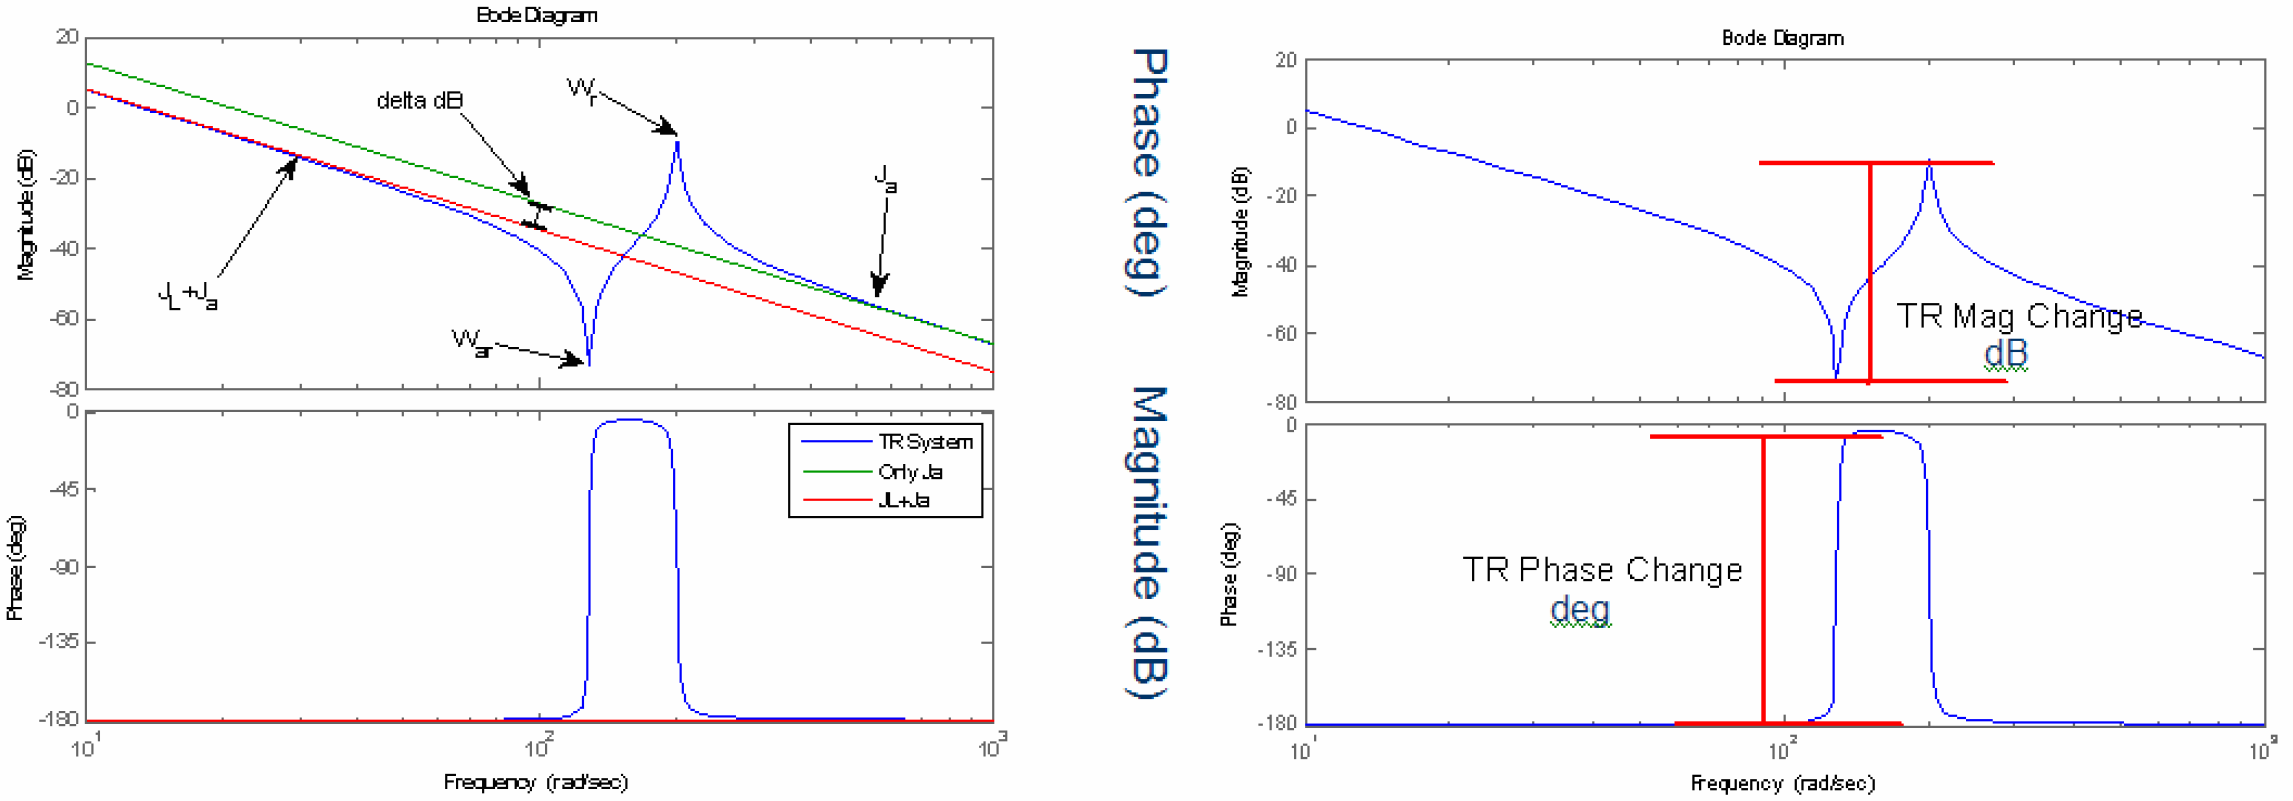
\includegraphics[width=1.0\columnwidth]{./pix/trshow.png}
  \caption{Frequency Response Plot of System with TR (from Eq. \ref{eq:ssTR}), System with no TR with
inertial load of $J_a$, and System with no TR and inertial load of $J_a+J_L$}
  \label{fig:trBode}
\end{figure}



The poles of a system with TR (\ref{eq:tf}) consists of a double pole at the origin and complex conjugate (CC) poles.  The CC poles are in the left half plane (LHP) as long as the following inequality is satisfied.

\begin{equation}
4K_c > B_c^2 \left( \frac{J_c+J_L}{J_aJ_L} \right)
\end{equation}

\noindent The system can represented in state space as
\noindent The system can represented in state space as

\begin{equation}\label{eq:ssTR}
\begin{array}{lllllll}

\left[
\begin{array}{l}
\ddot{\theta_a} 	\\ 
\dot{\theta_a}		\\
\ddot{\theta_L}	\\
\dot{\theta_L}
\end{array}
\right]



&


=

&

A

&

\left[
\begin{array}{l}
\dot{\theta_a} 	\\ 
\theta_a		\\
\dot{\theta_L}	\\
\theta_L
\end{array}
\right]

&

+

&

B

&

T(t)


\end{array}
\end{equation}


where


\begin{equation}
\begin{array}{lll}
A
&
=
&

\left[
\begin{array}{cccc}
\frac{-(B_a+B_c)}{J_a}   	& \frac{-K_c}{J_a}   	& \frac{B_c}{J_a}   		&	\frac{K_c}{J_a} \\
1 					& 0				& 0					&	0			\\
\frac{B_c}{J_L}			& \frac{K_c}{J_L}	& \frac{-(B_c+B_L)}{J_L}	& 	\frac{-K_c}{J_L} \\
0					& 0				& 0					&	1		
\end{array}

\right]


\end{array}
\end{equation}



\begin{equation}
\begin{array}{lllrrr}
B

&

=

&

\left[
\begin{array}{r}
J^{-1}_a 	\\ 
0		\\
0	\\
0
\end{array}
\right]
,
&
C
&
=
&
\left[
\begin{array}{cccc}
0 	&	1	&	0	&	0
\end{array}
\right]




\end{array}
\end{equation}

\noindent standard techniques show that the system is fully controllable and with the angular position $\theta_a$ being the only output is also fully observable.  The controllability and observability matrix are both full rank.




\cite{5686315}